\section{ЧАСТЬ 4. ОРГАНИЗАЦИОННО-ЭКОНОМИЧЕСКАЯ ЧАСТЬ}
\subsection{Оценка единовременных затрат на прототип}
Привод газоперекачивающего агрегата (ГПА) – сложное изделие с чрезвычайно широкой номенклатурой используемых материалов.
Точный расчет по всей номенклатуре крайне затруднителен, а на этапе эскизного проектирования – невозможен. Основной
вклад в затраты вносят дорогостоящие сплавы для горячей части двигателя (гранулированные ЭП741НП, жаропрочные для
охлаждаемых лопаток ЖС6К, ЖС6У, ЖС32) и легкие титановые сплавы для холодной части (ВТ3, ВТ6, ВТ8, ВТ9, АЛ4). Для
сравнительно ненапряженных температурных условий используются хромникелевые и нержавеющие стали и сплавы.

Для упрощения задачи, зная массу прототипа (6650 кг), закладываю коэффициент использования материала КИМ=0,05 и умножаю
на осредненную стоимость материалов (2500 р/кг). Для того, чтобы учесть затраты на оплату труда рабочих, на сумму затрат
на материалы вводится коэффициент 1,5.

Итого, получается стоимость прототипа:
$$
    Ц = 66500,05 \cdot 2500 р/кг \cdot 1,5 = 498750000 руб = 498,75 млн.руб
$$.

\subsection{Оценка снижения затрат в связи с доработкой конструкции}
В научно-исследовательской части настоящей выпускной квалификационной работы была усовершенствована конструкция
компрессора высокого давления: повышены напорности ступеней, в результате чего удалось уменьшить число ступеней с 7 до 5.
Была произведена оценка выигрыша в массе:
\begin{longtable}{|l|l|l|l|l|l|l|}
        \hline
        \textbf{№}&
        \textbf{\makecell{Масса \\ статора, \\ кг}}&
        \textbf{\makecell{Количество \\ лопаток \\ статора}}&
        \textbf{\makecell{Масса \\ лопаток \\ статора}}&
        \textbf{\makecell{Масса \\ ротора, \\ кг}}&
        \textbf{\makecell{Количество \\ лопаток \\ ротора}}&
        \textbf{\makecell{Масса \\ лопаток \\ ротора}}\\\hline
        \endhead
        1 & 23,6 & 23 & 0,3 & 37,1 & 25 & 0,28 \\\hline
        2 & 21,7 & 27 & 0,3 & 38,6 & 29 & 0,29 \\\hline
        \caption{Данные для оценки снижения массы двигателя в сравнении с прототипом} \label{tab:economics-mass-comparison}
    \end{longtable}
Экономия массы в сравнении с прототипом $\Delta m$, кг составила:
$$
    \Delta_m= \left(
        23,6 + 23 \cdot 0,3 + 37,1 + 25 \cdot 0,28
    \right) +
$$
$$
    + \left(
        21,7 + 27 \cdot 0,3 + 38,6 + 29 \cdot 0,29
    \right) = 151,4 \ кг
$$
Можно оценить снижение исходной массы материала для производства установки с учетом коэффициента использования материала:
$$
    \frac{\Delta_m}{КИМ} = \frac{151,4}{0,05} = 3028 \ кг.
$$
Следовательно, снижение затрат на материалы:
$$
    3028 \ кг \cdot 2500 \ р/кг = 7570000 \ руб.
$$
Принимая, что масса остальных деталей и узлов двигателя остается такой же, как в прототипе, вычисляем единовременные
затраты на проектируемый двигатель:
$$
    498750000 - 7570000 = 491180000 \ руб. = 491,18 \ млн.руб.
$$
\subsection{Оценка затрат на единицу мощности}
Одной из важнейших характеристик привода газоперекачивающего агрегата является мощность. С повышением требований к
параметрам цикла двигателя ужесточаются условия работы его узлов и деталей. Применяются сплавы, легированные
дорогостоящими металлами, гранулированные сплавы, повышается трудоемкость изготовления и сборки ДСЕ. Важно оценивать
затраты на единицу мощности. Оценка затрат на единицу мощности представлена в таблице 2
\begin{longtable}{|p{6cm}|c|c|}
    \hline
    \textbf{Параметр} &
    \textbf{Прототип} &
    \textbf{Проектируемый двигатель} \\\hline
    \endhead
    Мощность, МВт & 16 & 16 \\\hline
    Единовременные затраты, млн. руб. & 498,75 & 491,18 \\\hline
    Затраты на единицу мощности, млн. руб./МВт & 31,17 & 30,70 \\\hline
    \caption{Данные для оценки затрат на единицу мощности для прототипа и проектируемого двигателя} \label{tab:economics-unit-power}
    \end{longtable}
Анализ данных, представленных в таблице 2, показывает, что проектируемый двигатель является более выгодным с точки зрения
затрат на единицу мощности по сравнению с прототипом.

\subsection{Расчет затрат на эксплуатацию}
Заложен полный ресурс 100 тыс.ч. Межремонтный интервал – 25 тыс. ч. Затраты на один ремонт составляют 0,25 от единовременных затрат.
Таким образом получим стоимость одного ремонта двигателя $С_{рем}$:
\begin{longtable}{c c}
    Прототип & $498,75 \cdot 0,25=124,69$ млн.руб \\
    Проектируемый двигатель & $491,18 \cdot 0,25=122,80$ млн.руб \\
\end{longtable}
Цена газа для промышленных потребителей $Ц_{топл} = 4316 руб/(тыс \ м^3)$.
Примерный среднечасовой расход топлива проектируемого двигателя
$$
    G_т = 4,422 \ тыс \ м^3 / час.
$$
Можно посчитать среднегодовые затраты на топливо проектируемого двигателя
$$
    С_{топл}=G_т \cdot Ц_{топл} \cdot 8760 = 4,422 \cdot 4316 \cdot 8760 = 167,18 \ млн.руб./год.
$$
А также среднегодовые затраты на топливо прототипа
$$
    С_{топл \ прот} = G_{т \ прот} \cdot Ц_{топл} \cdot 8760 = 4,667 \cdot 4316 \cdot 8760 = 176,45 млн.руб./год.
$$
Введем коэффициент эксплуатационных затрат $К_{эксп} = 0,8$, связывающий среднегодовые затраты на регламентное и
техническое обслуживание и среднегодовые затраты на капитальный ремонт установки. В результате получим среднегодовые
затраты на регламентное и техническое обслуживание установки:
$$
    С_{эксп \ прот} = К_{эксп} \cdot С_{рем \ прот} \cdot 876025000 = 0,8 \cdot 124,69 \cdot 876025000 = 34,95 млн.руб \
$$
$$
    С_{эксп} = К_{эксп} \cdot С_{рем} \cdot 876025000 = 0,8 \cdot 122,80 \cdot 876025000 = 34,42 \ млн.руб.
$$

\begin{figure}[H]
    \centering
    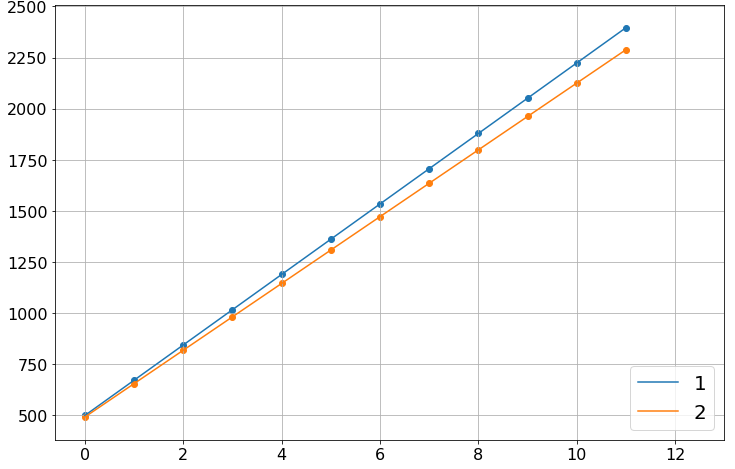
\includegraphics[scale=0.7]{cost}
    \caption{Суммарные затраты на прототип 1 и проектируемый двигатель 2 за 11 лет эксплуатации}
\end{figure}
Проведенная в исследовательской части дипломного проекта оптимизация цикла установки позволяет снизить единовременные
затраты за счет уменьшения стоимости компрессора высокого давления, а использование высокой температуры в камере сгорания
увеличивает экономичность двигателя в целом.